% IT5006 Phase 2 final report, version 4: teammates' v1, corrected and condensed with v3 content.
% Run Phase2/reports/phase2_final_evidence.py after updating saved results; it refreshes
% only the marked number and figure blocks below. This file compiles standalone.
\documentclass[12pt,a4paper]{article}
\usepackage[margin=0.8in]{geometry}
\usepackage[T1]{fontenc}
\usepackage{lmodern}
\usepackage{microtype}
\usepackage{booktabs}
\usepackage{array}
\usepackage{graphicx}
\usepackage{tikz}
\usepackage{float}
\usepackage{pgfplots}
\pgfplotsset{compat=1.16}
\usepackage{hyperref}
\hypersetup{colorlinks=true,linkcolor=blue,urlcolor=blue}
\setlength{\parindent}{0pt}
\setlength{\parskip}{0.4em}
\renewcommand{\arraystretch}{1.1}
% BEGIN GENERATED numbers -- refreshed by phase2_final_evidence.py
% Generated by reports/phase2_final_evidence.py: do not edit by hand.
\newcommand{\ActShare}{10}
\newcommand{\AllOrders}{96{,}272}
\newcommand{\AugModelNotPast}{107}
\newcommand{\AugRuleNotPast}{120}
\newcommand{\BacklogBasePR}{0.382}
\newcommand{\BacklogWins}{5}
\newcommand{\BacklogWithPR}{0.392}
\newcommand{\BadReviewLate}{62}
\newcommand{\BadReviewOnTime}{9}
\newcommand{\BadReviewRatio}{6.7}
\newcommand{\BlackFridayLate}{12}
\newcommand{\BusyGainMax}{31}
\newcommand{\BusyGainMin}{21}
\newcommand{\BusyRateMax}{21}
\newcommand{\BusyRateMin}{10}
\newcommand{\CalmGainMax}{24}
\newcommand{\CalmGainMin}{12}
\newcommand{\CalmRateMax}{5}
\newcommand{\CalmWindows}{W1 and W3}
\newcommand{\CarrierMean}{9.3}
\newcommand{\CarrierShare}{85}
\newcommand{\CheckoutBestMAE}{5.78}
\newcommand{\CheckoutBestName}{forest\_leaf20}
\newcommand{\CheckoutBestRMSE}{9.34}
\newcommand{\CheckoutBestRSq}{0.176}
\newcommand{\CheckoutImpAName}{numeric\_\_promised\_days}
\newcommand{\CheckoutImpAVal}{1.780}
\newcommand{\CheckoutImpBName}{logged\_\_distance\_km}
\newcommand{\CheckoutImpBVal}{1.111}
\newcommand{\CheckoutImpCName}{numeric\_\_route\_typical\_days}
\newcommand{\CheckoutImpCVal}{0.882}
\newcommand{\CheckoutImpKind}{coefficient (mean $|$weight$|$ over windows, numeric and engineered inputs; one-hot state/category dummies excluded from this ranking)}
\newcommand{\CheckoutMeanMAE}{7.21}
\newcommand{\CheckoutMeanRMSE}{10.67}
\newcommand{\CheckoutMeanRSq}{-0.078}
\newcommand{\CheckoutPR}{0.213}
\newcommand{\CheckoutRandTestMAE}{5.04}
\newcommand{\CheckoutRandTestRSq}{0.276}
\newcommand{\CheckoutRandValRSq}{0.259}
\newcommand{\CheckoutSelGap}{0.026}
\newcommand{\CheckoutSelGapSE}{0.028}
\newcommand{\CheckoutSelMAE}{5.81}
\newcommand{\CheckoutSelName}{ridge\_100}
\newcommand{\CheckoutSelRMSE}{9.40}
\newcommand{\CheckoutSelRSq}{0.167}
\newcommand{\CheckoutTestBias}{3.65}
\newcommand{\CheckoutTestMAE}{5.00}
\newcommand{\CheckoutTestRMSE}{6.41}
\newcommand{\CheckoutTestRSq}{-0.175}
\newcommand{\ClsBestName}{logistic\_c0.01}
\newcommand{\ClsCheckoutSelName}{logistic\_c0.01}
\newcommand{\ClsDefaultPR}{0.377}
\newcommand{\ClsPlainName}{logistic\_unregularized}
\newcommand{\ClsPlainPR}{0.371}
\newcommand{\ClsSelGap}{0.000}
\newcommand{\ClsSelGapSE}{0.000}
\newcommand{\ClsSelName}{logistic\_c0.01}
\newcommand{\ClsTestFone}{0.29}
\newcommand{\ClsTestLate}{3.5}
\newcommand{\ClsTestMCC}{0.29}
\newcommand{\ClsTestPR}{0.49}
\newcommand{\ClsTestPrec}{19.6}
\newcommand{\ClsTestROC}{0.86}
\newcommand{\ClsTestRec}{56}
\newcommand{\CohortOrders}{96{,}272}
\newcommand{\DisruptLateShare}{72}
\newcommand{\EtaTestDeliveryMean}{8.8}
\newcommand{\EtaTestDeliverySD}{5.9}
\newcommand{\EtaTestOrders}{19{,}230}
\newcommand{\EtaTrainDeliveryMean}{13.3}
\newcommand{\EtaTrainDeliverySD}{9.8}
\newcommand{\EtaTrainOrders}{75{,}039}
\newcommand{\ExcludedOrders}{198}
\newcommand{\FebMarLate}{17}
\newcommand{\FrozenTestCaught}{370}
\newcommand{\FullDailyActiveDays}{81}
\newcommand{\FullDailyBeforePromise}{191}
\newcommand{\FullDailyCaught}{388}
\newcommand{\FullDailyCaughtOpen}{387}
\newcommand{\FullDailyCaughtPerDay}{5}
\newcommand{\FullDailyExpiredCaught}{197}
\newcommand{\FullDailyFlagged}{1{,}988}
\newcommand{\FullDailyLate}{705}
\newcommand{\FullDailyMedianFlagged}{27}
\newcommand{\FullDailyOrders}{19{,}534}
\newcommand{\FullDailyPninetyFlagged}{40}
\newcommand{\FullDailyPrecision}{19.5}
\newcommand{\FullDailyRecall}{55.0}
\newcommand{\FullDailyRecallRound}{55}
\newcommand{\GainFiveModel}{46}
\newcommand{\GainOneModel}{20}
\newcommand{\GainTenModel}{56}
\newcommand{\GainTwentyModel}{70}
\newcommand{\HandoverBestMAE}{5.10}
\newcommand{\HandoverBestName}{ridge\_100}
\newcommand{\HandoverBestRMSE}{8.41}
\newcommand{\HandoverBestRSq}{0.338}
\newcommand{\HandoverImpAName}{numeric\_\_handover\_days}
\newcommand{\HandoverImpAVal}{3.436}
\newcommand{\HandoverImpBName}{logged\_\_distance\_km}
\newcommand{\HandoverImpBVal}{1.218}
\newcommand{\HandoverImpCName}{numeric\_\_promise\_slack}
\newcommand{\HandoverImpCVal}{1.003}
\newcommand{\HandoverImpKind}{coefficient (mean $|$weight$|$ over windows, numeric and engineered inputs; one-hot state/category dummies excluded from this ranking)}
\newcommand{\HandoverMeanMAE}{7.21}
\newcommand{\HandoverMeanRMSE}{10.67}
\newcommand{\HandoverMeanRSq}{-0.078}
\newcommand{\HandoverRandTestMAE}{4.34}
\newcommand{\HandoverRandTestRSq}{0.411}
\newcommand{\HandoverRandValRSq}{0.386}
\newcommand{\HandoverRuleMAE}{5.30}
\newcommand{\HandoverRuleRSq}{0.337}
\newcommand{\HandoverSelGap}{0.000}
\newcommand{\HandoverSelGapSE}{0.000}
\newcommand{\HandoverSelMAE}{5.10}
\newcommand{\HandoverSelName}{ridge\_100}
\newcommand{\HandoverSelRMSE}{8.41}
\newcommand{\HandoverSelRSq}{0.338}
\newcommand{\HandoverTestBias}{2.87}
\newcommand{\HandoverTestMAE}{3.97}
\newcommand{\HandoverTestRMSE}{5.44}
\newcommand{\HandoverTestRSq}{0.154}
\newcommand{\ImpADisplay}{slack shortfall}
\newcommand{\ImpADrop}{0.083}
\newcommand{\ImpAName}{slack\_shortfall}
\newcommand{\ImpBDisplay}{elapsed time}
\newcommand{\ImpBDrop}{0.056}
\newcommand{\ImpBName}{handover\_days}
\newcommand{\ImpCDisplay}{remaining slack}
\newcommand{\ImpCDrop}{0.032}
\newcommand{\ImpCName}{remaining\_slack}
\newcommand{\ImpDDisplay}{route\_transit\_90d\_at\_handover}
\newcommand{\ImpDDrop}{0.030}
\newcommand{\ImpDName}{route\_transit\_90d\_at\_handover}
\newcommand{\ImpEDisplay}{promised\_days}
\newcommand{\ImpEDrop}{0.026}
\newcommand{\ImpEName}{promised\_days}
\newcommand{\ImpFDisplay}{distance\_km}
\newcommand{\ImpFDrop}{0.016}
\newcommand{\ImpFName}{distance\_km}
\newcommand{\JunModelNotPast}{31}
\newcommand{\JunRuleNotPast}{31}
\newcommand{\LadderCheckoutMAE}{5.81}
\newcommand{\LadderCheckoutMinRSq}{0.060}
\newcommand{\LadderCheckoutRSq}{0.167}
\newcommand{\LadderElapsedMAE}{5.11}
\newcommand{\LadderElapsedMinRSq}{0.222}
\newcommand{\LadderElapsedRSq}{0.335}
\newcommand{\LadderHandoverMAE}{5.10}
\newcommand{\LadderHandoverMinRSq}{0.227}
\newcommand{\LadderHandoverRSq}{0.338}
\newcommand{\LadderTransitMAE}{5.68}
\newcommand{\LadderTransitMinRSq}{0.078}
\newcommand{\LadderTransitRSq}{0.214}
\newcommand{\LaterLift}{5.6}
\newcommand{\LaterLossPct}{5}
\newcommand{\LaterModelCaught}{377}
\newcommand{\LaterRuleCaught}{398}
\newcommand{\MonthlyRuleTestCaught}{394}
\newcommand{\MonthlyRuleValCaught}{1{,}074}
\newcommand{\MonthlyTestCaught}{379}
\newcommand{\MonthlyValCaught}{1{,}334}
\newcommand{\NormalLate}{4}
\newcommand{\OosGainPct}{14}
\newcommand{\OosModelCaught}{1{,}246}
\newcommand{\OosRuleCaught}{1{,}094}
\newcommand{\OosWins}{3}
\newcommand{\PastPromiseLateRate}{99.4}
\newcommand{\PastPromiseTest}{29.5}
\newcommand{\PastPromiseVal}{4.1}
\newcommand{\PastPromiseWinMax}{12}
\newcommand{\PastPromiseWinMin}{1}
\newcommand{\PrecFiveModel}{32}
\newcommand{\PrecOneModel}{69}
\newcommand{\PrecTenModel}{20}
\newcommand{\PrecTwentyModel}{12}
\newcommand{\PromAug}{15.2}
\newcommand{\PromJul}{19.7}
\newcommand{\PromJun}{27.8}
\newcommand{\PromSpanMax}{28}
\newcommand{\PromSpanMin}{22}
\newcommand{\QuarterlyValCaught}{1{,}256}
\newcommand{\RatedOrders}{95{,}627}
\newcommand{\RepeatAfterLate}{2.5}
\newcommand{\RepeatAfterOnTime}{3.0}
\newcommand{\RepeatShare}{3.0}
\newcommand{\RuleGapHigh}{0.072}
\newcommand{\RuleGapLow}{0.057}
\newcommand{\RuleGapPR}{0.064}
\newcommand{\RuleRecallTen}{59}
\newcommand{\RuleTestFone}{0.31}
\newcommand{\RuleTestPR}{0.52}
\newcommand{\RuleTestPrec}{20.7}
\newcommand{\RuleTestROC}{0.88}
\newcommand{\RuleTestRec}{59}
\newcommand{\RuleValPR}{0.328}
\newcommand{\ShapeBeatsRuleWindows}{5}
\newcommand{\ShapeRecallWith}{56}
\newcommand{\ShapeRecallWithout}{46}
\newcommand{\ShapeTestWith}{0.49}
\newcommand{\ShapeTestWithout}{0.25}
\newcommand{\ShapeThreeWins}{5}
\newcommand{\ShapeValNoThree}{0.378}
\newcommand{\ShapeValWith}{0.392}
\newcommand{\ShapeValWithout}{0.379}
\newcommand{\ShapeWinsWindows}{5}
\newcommand{\ShortCut}{14.5}
\newcommand{\ShortShareAug}{56}
\newcommand{\ShortTestPRModel}{0.169}
\newcommand{\ShortTestPRRule}{0.195}
\newcommand{\ShortValLateMax}{53}
\newcommand{\ShortValLateMin}{3}
\newcommand{\ShortValModelWins}{3}
\newcommand{\TestAugActed}{631}
\newcommand{\TestAugCaught}{232}
\newcommand{\TestAugLateCount}{393}
\newcommand{\TestAugOrders}{6{,}306}
\newcommand{\TestJulActed}{612}
\newcommand{\TestJulCaught}{113}
\newcommand{\TestJulLateCount}{207}
\newcommand{\TestJulOrders}{6{,}119}
\newcommand{\TestJunActed}{605}
\newcommand{\TestJunCaught}{31}
\newcommand{\TestJunLateCount}{70}
\newcommand{\TestJunOrders}{6{,}050}
\newcommand{\TestMayActed}{76}
\newcommand{\TestMayCaught}{1}
\newcommand{\TestMayLateCount}{2}
\newcommand{\TestMayOrders}{755}
\newcommand{\TestOrders}{19{,}230}
\newcommand{\TotalMean}{12.6}
\newcommand{\TrainPromised}{24.3}
\newcommand{\UniqueCustomers}{93{,}159}
\newcommand{\ValBestPR}{0.392}
\newcommand{\ValGainMax}{31}
\newcommand{\ValGainMin}{12}
\newcommand{\ValSelPR}{0.392}
\newcommand{\ValSelROC}{0.780}
\newcommand{\ValSelRecallTen}{37}
\newcommand{\WFiveModelCaught}{469}
\newcommand{\WFiveRuleCaught}{357}
\newcommand{\WTwoModelCaught}{341}
\newcommand{\WTwoRuleCaught}{271}
\newcommand{\WalkMaxGap}{0.000}
\newcommand{\WalkSame}{3}
% END GENERATED numbers

\begin{document}
\begin{titlepage}
\centering
\vspace*{0.8cm}
\IfFileExists{NUS_logo_full-horizontal.jpg}{%
  
\includegraphics[width=0.6\textwidth]{NUS_logo_full-horizontal.jpg}\par
}{%
  \IfFileExists{reports/NUS_logo_full-horizontal.jpg}{%
    \includegraphics[width=0.6\textwidth]{reports/NUS_logo_full-horizontal.jpg}\par
  }{%
    {\Huge\bfseries NUS\par}
    \vspace{0.2cm}
    {\large National University of Singapore\par}
    \vspace{1.8cm}
  }%
}
\vspace{1.6cm}
{\LARGE\bfseries Keeping Delivery Promises at Olist\par}
\vspace{0.4cm}
{\large Two-stage Delivery-time Estimation and Late-order Prioritisation at Carrier Handover\par}
\vspace{1.3cm}
{\large\bfseries IT5006 Phase 2\par}
\vspace{0.3cm}
{\large AY2026/27 Semester 1\par}
\vspace{1.4cm}
{\large\bfseries Group 6\par}
\vspace{0.6cm}
{\normalsize
CHAI WEI NI, WINNIE (A0172261M)\par
LE TRUNG HIEU (A0286973H)\par
LIANG ZIYAN (A0291506E)\par
LUM ZI YUAN JOSHUA (A0108499N)\par
SHAH PRATIK (A0211041H)\par
YUAN JIAYI (A0177893H)\par
}
\vfill
{\footnotesize Code and notebooks: \url{https://github.com/YuanJiayi/Team6_IT5006_Ecommerce_Analytics_AY2627Sem1}}\par
\vspace*{0.5cm}
\end{titlepage}


\section*{Executive Summary}
Late deliveries hurt Olist's reviews: \BadReviewLate{}\% of late orders receive a one- or two-star review, against \BadReviewOnTime{}\% of on-time orders. Our aim is to help the delivery operations team act on late orders early. When a seller hands a parcel to the carrier, two models help. The \textbf{classifier} ranks that day's parcels by their risk of missing the date the customer was promised. The \textbf{regression} estimates how many more days each delivery will take. Figure~\ref{fig:workflow} shows where both sit in an order's journey.

\textbf{Validation results.} Across five chronological validation windows:

\begin{itemize}\setlength{\itemsep}{0pt}
\item \textbf{Delivery-time estimate.} Our chosen regression is a ridge regression ($\alpha=100$), selected on validation from linear and tree-based models. At checkout it has an MAE of \CheckoutSelMAE{} days. Once the carrier has the parcel, we update the estimate using how long the order has already taken, and the MAE falls to \HandoverSelMAE{} days. The update is more accurate in every validation period, and it beats a simple rule of thumb, days so far plus the route's usual carrier time (MAE \HandoverRuleMAE{} days).
\item \textbf{Late warning.} Without a model, staff could rank parcels by their spare time: the days left until the promised date, minus how long the carrier usually takes on that route. A parcel promised in 6 days on a route that usually takes 8 has $-2$ days of spare time and goes near the top. Our chosen classifier, a regularised logistic regression ($C=0.01$) and the best of the linear and tree-based candidates on validation, produces a better list. Checking the same number of parcels, it finds \ValGainMin{}--\ValGainMax{}\% more late orders than this rule in every validation period.
\end{itemize}

Together, they give operations one daily list, produced while there is still time to act: which parcels to check first, and roughly when each will arrive.

\textbf{Test-set results.} The handover regression reduces MAE from \CheckoutTestMAE{} days at checkout to \HandoverTestMAE{} days, but overestimates delivery time by \HandoverTestBias{} days on average as deliveries become faster. For the classifier, the top 10\% of each month's list holds \GainTenModel{}\% of late orders, against 10\% for a random list. The spare-time rule does better, mainly in August, when \ShortShareAug{}\% of orders have promises under \ShortCut{} days versus about 10\% of training orders. Monthly retraining helps slightly but does not close that gap; the rule is a useful fallback while conditions change faster than the model can learn from completed deliveries.

\section*{Business Problem and Model Roles}
The carrier leg, from handover to customer, averages \CarrierMean{} of the \TotalMean{} mean total delivery days and contributes \CarrierShare{}\% of total delivery-time variance in a covariance-based decomposition. Most of the uncertainty a customer experiences therefore arises after the seller hands the parcel to the carrier. Among \RatedOrders{} delivered orders with a review, \BadReviewLate{}\% of late orders received a bad review (score 1 or 2), against \BadReviewOnTime{}\% of on-time orders, so a late parcel is \BadReviewRatio{} times as likely to earn one. Phase 1 also found delivery time rising from 5.9 to 18.5 days across distance sextiles, and a backlog persisting after the November sales peak. These observations motivate our route and recent-history features.

The decision point is carrier handover, when review capacity is limited and the customer's date is already set. The classifier answers \emph{which orders to examine first}; the regression answers \emph{how much delivery time remains} for an order being reviewed, so the two outputs are complementary rather than redundant. The checkout fit is the earlier benchmark for measuring the value of handover information. We evaluate forecast error, late-order ranking, and the workload implied by a sample review list.

\section*{Data Preparation and Point-in-time Evaluation}
From 99,441 recorded Olist orders, 96,470 were delivered with both actual and estimated delivery dates; \ExcludedOrders{} lack a valid purchase-to-carrier-to-customer sequence, leaving \CohortOrders{} orders for both models. Of these, \EtaTrainOrders{} had outcomes known before the 26 May 2018 cutoff, \EtaTestOrders{} were purchased on or after it, and 2,003 earlier purchases had outcomes unavailable at the cutoff and were excluded from fitting and testing. A late order arrives after Olist's estimated \emph{calendar date}; arrival on that date is on time. Results therefore describe eventually delivered orders with a valid handover, not every purchase.

\textbf{One row per order.} Orders are joined to customers, items, products, sellers and payments on their relevant keys, with item and payment rows aggregated before modelling; where an order involves several sellers, we use the furthest one. Geolocation observations are reduced to median ZIP-prefix coordinates, after removing 42 implausible points, so that a single order is not counted several times over. The resulting Haversine distance is a straight-line geographic proxy, similar to the origin--destination distance that de Araujo and Etemad use for last-mile forecasting~\cite{dearaujo2021}. Missing numeric values are filled with the training fold's median, and missing categorical values are given an explicit "unknown" level. For the repeat-customer figures we use \texttt{customer\_unique\_id} rather than the order-specific \texttt{customer\_id}; because these \UniqueCustomers{} customers come from this narrower delivery cohort, the count differs from Phase 1's broader EDA cohort.

\textbf{Temporal split, not random.} The test set holds every order purchased from 26 May 2018 onward (\TestOrders{} orders). Earlier orders form five chronological validation windows, from 22 September 2017 to 26 March 2018. Each window is fitted only on purchases whose delivery outcome was recorded before the window begins. Validation stops on 26 March, leaving a 60-day margin before the test cutoff for delivery outcomes to mature; without it, long-running orders near the cutoff would still be in transit, and lateness would look artificially low. Each window keeps its natural late rate rather than having it smoothed away by stratification. A random split would let the model learn from orders still in transit at prediction time and would hide how conditions shift between periods; time-ordered validation avoids both~\cite{bergmeir2012}.

\textbf{Feature hypotheses and availability.} Phase 1's review found that route geography, order timing and order complexity were all related to delivery time, and it cautioned that information from an order's still-unfinished stages must not become predictors. Table~\ref{tab:feature-rationale} turns those observations into a timed feature contract.

\begin{table}[ht]
\centering\footnotesize
\caption{Why the engineered inputs belong in each prediction stage. Historical means use outcomes completed strictly before the relevant prediction time.}
\label{tab:feature-rationale}
\begin{tabular}{@{}p{2.5cm}p{6.15cm}p{7cm}@{}}
\toprule
Stage and signal & Construction & Rationale and boundary \\
\midrule
Checkout: route & Approximate seller--buyer distance; seller/customer state; past route delivery mean, shrunk toward the prior overall mean. & Phase 1's distance gradient and historical transit summaries in Gibellini et al.~\cite{gibellini2024} motivate our route-history feature; our grouping and shrinkage use earlier Olist deliveries only. \\
Checkout: order & Purchase hour/weekday; item and seller counts; price, freight, weight and volume. Skewed numeric inputs use $\log(1+x)$ for linear models. & Salari et al. use order hour, weekday and item counts in delivery forecasting~\cite{salari2022}; our log scaling limits leverage from large values. \\
Checkout: promise & Olist's stored promised days and promise minus historical route mean. & The late label is relative to this date. We assume it was visible at checkout; the CSV has no promise-revision history. \\
Handover: progress & Observed elapsed/approval days and recent 90-day route carrier time for regression; remaining slack (promised days minus elapsed days minus expected transit) for classification. & Gibellini et al. use observed shipment state and historical time aggregates~\cite{gibellini2024}. Our inputs use only outcomes known by handover, never this order's delivery. \\
Handover: slack shortfall & Whether the promised date had already passed at handover (yes/no); how many days slack is below zero (0 if positive). & Risk jumps once slack runs out. A logistic model treats slack as a straight line, so these inputs let it capture that jump; trees can split there without them. \\
Handover: regional backlog & Difference between $\log(1+B)$ for today's open buyer-state count and for its mean at eight earlier weekly snapshots; exclude the order being scored. & Phase 1 found backlog persisting after the November sales peak. More outstanding orders than usual may signal congestion beyond route history. \\
\bottomrule
\end{tabular}
\end{table}

\textbf{Leakage and reproducibility.} Preprocessing is fitted inside fold-specific Pipelines, so imputation, one-hot encoding and, for linear models, scaling are learned from the fitting rows only. Purchase hour is encoded cyclically for the linear models, while the tree-based models use the raw numeric value. Route and seller histories draw only on earlier orders whose outcomes were already recorded, and an order's own actual delivery, review and later status are never included as predictors. The stored promise, payment details and static ZIP map lack historical snapshot timestamps, so their checkout availability is an assumption rather than verified fact. Everything needed to reproduce the model comparisons (the random seed 42, the feature contracts, the split assignments and both model scripts) is in \texttt{Phase2/} in the accompanying GitHub repository. Appendix~\ref{app:gx} reports the Great Expectations checks on the prepared order table.

\begin{figure}[ht]
\centering
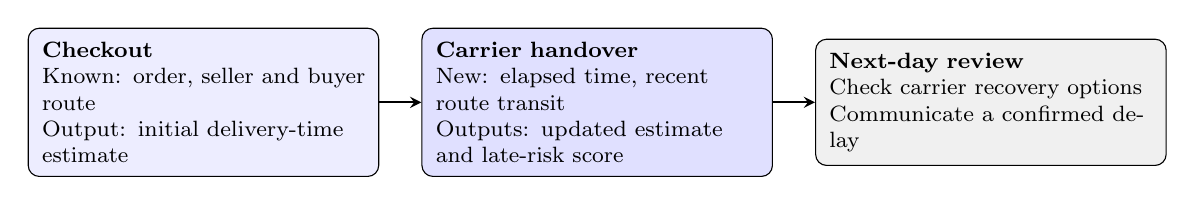
\begin{tikzpicture}[>=stealth,every node/.style={font=\footnotesize}]
\node[draw,rounded corners,fill=blue!7,align=left,text width=4.1cm,inner sep=5pt] (checkout) at (0,0) {\textbf{Checkout}\par Known: order, seller and buyer route\par Output: initial delivery-time estimate};
\node[draw,rounded corners,fill=blue!12,align=left,text width=4.1cm,inner sep=5pt] (handover) at (5.0,0) {\textbf{Carrier handover}\par New: elapsed time, recent route transit\par Outputs: updated estimate and late-risk score};
\node[draw,rounded corners,fill=gray!12,align=left,text width=4.1cm,inner sep=5pt] (action) at (10.0,0) {\textbf{Next-day review}\par Check carrier recovery options\par Communicate a confirmed delay};
\draw[->,thick] (checkout.east) -- (handover.west);
\draw[->,thick] (handover.east) -- (action.west);
\end{tikzpicture}
\caption{Prediction points and proposed action. Olist's original customer date anchors the late-risk label; delivery outcomes enter later model fits only after they are recorded.}
\label{fig:workflow}
\end{figure}

\section*{Model 1: Two-stage Delivery-time Estimate (Regression)}
\textbf{Task and features.} Both stages predict days from purchase to delivery for the same orders. Checkout uses 20 order, route and seller inputs available at purchase. Handover adds three feature types:
\begin{enumerate}\setlength{\itemsep}{0pt}
\item \textbf{Elapsed days} since purchase show how much of the total delivery time has already passed.
\item \textbf{Approval days} show how much of that time passed before payment approval, distinguishing an early processing delay from later fulfilment time. We use this only when approval was recorded by handover.
\item \textbf{Recent route carrier time} estimates the journey still ahead from deliveries completed on the same seller-state--customer-state route in the previous 90 days. Sparse routes are smoothed toward the overall mean. This history is available at checkout and updated at handover.
\end{enumerate}
Subtracting elapsed days from the handover prediction gives the reviewer an estimate of remaining delivery time. Table~\ref{tab:ladder} holds ridge (\(\alpha=100\)) fixed: it adds route history first, adds elapsed and approval days together, then refreshes route history at handover. MAE falls from \LadderCheckoutMAE{} to \LadderHandoverMAE{} days. The table does not isolate a separate gain from approval days.

\begin{table}[ht]
\centering\small
\caption{Information ladder: Ridge regression (\(\alpha=100\)) throughout, same orders at every rung, mean over five validation windows.}
\label{tab:ladder}
\begin{tabular}{@{}lrrr@{}}
\toprule
Rung & MAE (days) & \(R^2\) & Lowest-window \(R^2\) \\
\midrule
Checkout (20 original inputs) & \LadderCheckoutMAE{} & \LadderCheckoutRSq{} & \LadderCheckoutMinRSq{} \\
+ route history known at checkout & \LadderTransitMAE{} & \LadderTransitRSq{} & \LadderTransitMinRSq{} \\
+ elapsed and approval days at handover & \LadderElapsedMAE{} & \LadderElapsedRSq{} & \LadderElapsedMinRSq{} \\
Handover: refresh route history & \LadderHandoverMAE{} & \LadderHandoverRSq{} & \LadderHandoverMinRSq{} \\
\bottomrule
\end{tabular}
\end{table}

\textbf{Candidates and selection.} We select on MAE because it measures average forecast error in days. RMSE gives more weight to large errors, while $R^2$ measures fit against each period's mean. Table~\ref{tab:regression-family-summary} starts with a training-mean benchmark, plain linear regression and a single decision tree, then compares ridge and tree ensembles. The tree models test whether the non-linear effects suggested in our Phase 1 review improve forecasts. At checkout, the forest has the lowest MAE, but ridge is close. At handover, ridge has the lowest MAE and also beats a simple rule that predicts total delivery time as days elapsed since purchase plus the route's recent average carrier time.

% BEGIN GENERATED fig_regression_family_summary -- refreshed by phase2_final_evidence.py
\begin{table}[ht]
\centering\small
\caption{Regression comparison: mean MAE in days over five chronological validation windows. Lower is better. Full configurations are in Appendix Table~\ref{tab:app-regression}.}
\label{tab:regression-family-summary}
\begin{tabular}{@{}llrr@{}}
\toprule
Family & Configuration & Checkout & Handover \\
\midrule
Benchmark & Training mean & 7.21 & 7.21 \\
Linear & Plain linear regression & 5.86 & 5.15 \\
Linear & Ridge regression (selected) & 5.81 & 5.10 \\
Tree-based & Single decision tree & 7.79 & 6.84 \\
Tree-based & Tuned decision tree & 5.93 & 5.31 \\
Tree-based & Random forest & 5.78 & 5.35 \\
Tree-based & Gradient boosting & 5.83 & 5.21 \\
Benchmark & Elapsed time + route rule & -- & 5.30 \\
\bottomrule
\end{tabular}
\end{table}
% END GENERATED fig_regression_family_summary

For the final choice, we adapt the one-standard-error simplicity rule~\cite{james2013}: prefer a simpler candidate when its validation MAE is within one paired standard error of the best. At checkout, the forest beats ridge by only \CheckoutSelGap{} days, less than the paired SE of \CheckoutSelGapSE{}, so we choose ridge (\(\alpha=100\)). At handover, the same ridge has the lowest validation MAE; combining it with boosting offers no gain. The SE is approximate across five chronological windows. Appendix Table~\ref{tab:app-regression} shows every candidate.

\begin{figure}[ht]
\centering
% BEGIN GENERATED fig_ladder -- refreshed by phase2_final_evidence.py
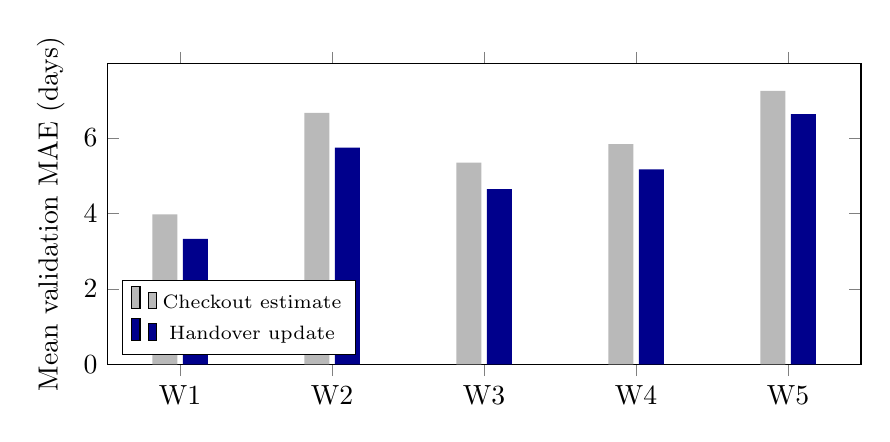
\begin{tikzpicture}
\begin{axis}[width=0.92\linewidth,height=5.4cm,ybar,bar width=9pt,ymin=0,ylabel={Mean validation MAE (days)},
 symbolic x coords={W1,W2,W3,W4,W5},xtick=data,enlarge x limits=0.12,legend style={at={(0.02,0.03)},anchor=south west,font=\scriptsize}]
\addplot[fill=gray!55,draw=none] coordinates {(W1,3.97) (W2,6.66) (W3,5.34) (W4,5.83) (W5,7.24)};
\addplot[fill=blue!55!black,draw=none] coordinates {(W1,3.32) (W2,5.74) (W3,4.64) (W4,5.16) (W5,6.63)};
\legend{Checkout estimate,Handover update}
\end{axis}
\end{tikzpicture}
% END GENERATED fig_ladder
\caption{Mean validation MAE by window, checkout estimate against the handover update (selected models). The handover update beats the checkout estimate in every window, including the higher-lateness windows.}
\label{fig:ladder}
\end{figure}

\textbf{Test-set results.} The handover regression has an MAE of \HandoverTestMAE{} days and a positive $R^2$ of \HandoverTestRSq{}. Using the information available at handover improves on the checkout estimate, whose MAE is \CheckoutTestMAE{} days and $R^2$ is \CheckoutTestRSq{}. The updated estimate is therefore more useful when staff review an order, though it still predicts \HandoverTestBias{} days too long on average (Appendix Figure~\ref{fig:test-bias}).

The checkout result needs context. We suspect temporal data drift: mean delivery time fell from \EtaTrainDeliveryMean{} days in training to \EtaTestDeliveryMean{} days in the test set. The checkout model overpredicted by \CheckoutTestBias{} days on average. Its RMSE of \CheckoutTestRMSE{} days exceeded the test set's \EtaTestDeliverySD{}-day standard deviation. Because $R^2$ compares squared prediction error with variation around the test-set mean, this gives a negative $R^2$: the model performed worse than that hindsight mean benchmark. The shift plausibly contributed to the overprediction, but these results cannot establish it as the only cause.

\textbf{What drives the estimate.} Among scaled numeric inputs, the largest mean absolute ridge coefficients at checkout are for promised days (\CheckoutImpAVal{}), distance (\CheckoutImpBVal{}) and typical route delivery time (\CheckoutImpCVal{}). At handover, elapsed time has the largest coefficient (\HandoverImpAVal{}), while distance remains relevant. The model thus updates the forecast for time already spent without treating all routes alike. Because predictors are correlated, coefficient size describes the fit rather than a causal effect.

\section*{Model 2: The Late Warning (Classification)}
\textbf{Task and features.} At carrier handover, the classifier ranks orders by their risk of arriving after Olist's existing promised date. The promise and handover time are known then; the outcome is known only after delivery. Four engineered features describe the time available and current delivery conditions:
\begin{enumerate}\setlength{\itemsep}{0pt}
\item \textbf{Remaining slack:} promised days minus days elapsed since purchase minus expected carrier time. The estimate uses deliveries completed in the preceding 90 days on the same seller-state--customer-state route, smoothed toward the overall mean for sparse routes. Less slack means the usual carrier journey leaves less room to meet the promise.
\item \textbf{Promise already passed:} an indicator of whether the promised date had elapsed by handover. This separates orders that have already missed the date from those that still have time for recovery.
\item \textbf{Slack shortfall:} the negative part of remaining slack: the number of days by which expected carrier time exceeds the time left until the promise, or zero if there is enough time. An order with five days to spare is a different operational situation from one expected to miss by five days. Risk may rise faster as that shortfall grows. This feature lets logistic regression learn a different effect for each day below zero slack, rather than use the same log-odds change on both sides.
\item \textbf{Relative buyer-state backlog:} the current number of open orders for buyers in the same state, compared with its average at eight earlier weekly snapshots. Both counts exclude the order being scored and use only events known by handover. A busy state is not necessarily congested; an unusually high backlog relative to that state's own recent level may signal pressure on delivery capacity.
\end{enumerate}
Operations could sort handovers by remaining slack and review the smallest values first. We call this the \emph{remaining-slack rule}; it serves as a benchmark and a temporary fallback when conditions shift. With backlog held fixed, adding the three slack features together raises mean validation PR-AUC from \ShapeValNoThree{} to \ValSelPR{} across all \ShapeThreeWins{} windows. With the slack features held fixed, adding relative buyer-state backlog raises PR-AUC from \BacklogBasePR{} to \BacklogWithPR{}, again across all \BacklogWins{} windows.

\textbf{Metric and model choice.} Late rates range from 4\% to 21\% across validation windows, so accuracy could reward predicting nearly everything on time. We select by PR-AUC because it summarises precision (the share of reviewed orders that are late) and recall (the share of late orders found) across review-list sizes~\cite{saito2015}. When most orders are on time, ROC-AUC alone can look strong even if a short review list has low precision; we report it as a complement, alongside top-list recall. Each window's late rate is its random-ranking PR-AUC reference. We compare two broad families: linear models, starting with plain logistic regression, and tree-based models, starting with a single decision tree (Table~\ref{tab:family-summary}). Regularisation raises logistic PR-AUC from \ClsPlainPR{} to \ValSelPR{}. The forest and boosting candidates do not improve on it, so we choose regularised logistic regression ($C=0.01$).

% BEGIN GENERATED fig_family_summary -- refreshed by phase2_final_evidence.py
\begin{table}[ht]
\centering\small
\caption{Classification comparison, mean over five chronological validation windows. Full configurations are in Appendix Table~\ref{tab:app-classifier}.}
\label{tab:family-summary}
\begin{tabular}{@{}llrr@{}}
\toprule
Family & Configuration & PR-AUC & ROC-AUC \\
\midrule
Linear & Plain logistic regression & 0.371 & 0.747 \\
Linear & Regularised logistic regression & 0.392 & 0.780 \\
Tree-based & Single decision tree & 0.140 & 0.567 \\
Tree-based & Tuned decision tree & 0.320 & 0.705 \\
Tree-based & Random forest & 0.373 & 0.744 \\
Tree-based & Gradient boosting & 0.363 & 0.741 \\
Benchmark & Remaining-slack rule & 0.328 & 0.697 \\
\bottomrule
\end{tabular}
\end{table}
% END GENERATED fig_family_summary

\textbf{Validation and interpretation.} We illustrate a fixed workload by reviewing the top \ActShare{}\% of each ranked list: one in ten handovers. This is a comparison setting, not an estimate of staffing capacity. At that share, the model finds more late orders than the remaining-slack rule in all five validation windows (Table~\ref{tab:period-value}); its mean PR-AUC is \ValSelPR{} against \RuleValPR{}. Validation permutation importance~\cite{breiman2001} shows the largest PR-AUC drops for \ImpADisplay{} (\ImpADrop{}), \ImpBDisplay{} (\ImpBDrop{}) and \ImpCDisplay{} (\ImpCDrop{}). The backlog comparison above establishes its additional ranking value even if other inputs carry more of the overall signal. Importance describes the fitted model, not causal effects. Training, validation and test-set summaries, curves and confusion counts appear in Appendix~\ref{app:diag}.

% BEGIN GENERATED fig_period_value -- refreshed by phase2_final_evidence.py
\begin{table}[ht]
\centering\small
\caption{Model against the remaining-slack rule at the same workload: the top \ActShare{}\% of each validation window, or of each purchase month in the test set (26 May--August 2018). A random list would catch \ActShare{}\% of late orders.}
\label{tab:period-value}
\begin{tabular}{@{}lrrrrrrr@{}}
\toprule
& & Late already & \multicolumn{2}{c}{PR-AUC} & \multicolumn{3}{c}{Late orders caught} \\
\cmidrule(lr){4-5}\cmidrule(l){6-8}
Period & Late rate & past date & Model & Rule & Model & Rule & Random \\
\midrule
W1 & 4.1\% & 12\% & 0.378 & 0.354 & 164 & 132 & 31 \\
W2 & 13.8\% & 6\% & 0.430 & 0.343 & 341 & 271 & 105 \\
W3 & 4.8\% & 7\% & 0.282 & 0.256 & 126 & 112 & 36 \\
W4 & 9.9\% & 3\% & 0.370 & 0.301 & 274 & 227 & 75 \\
W5 & 20.7\% & 1\% & 0.502 & 0.386 & 469 & 357 & 158 \\
Test set & 3.5\% & 29\% & 0.489 & 0.519 & 377 & 398 & 67 \\
\bottomrule
\end{tabular}
\end{table}
% END GENERATED fig_period_value

\textbf{Test-set results.} At the same \ActShare{}\% review share, the model finds \ClsTestRec{}\% of late orders with \ClsTestPrec{}\% precision, well above the \ClsTestLate{}\% late rate of a random list. The rule finds more late orders than the model (\LaterRuleCaught{} versus \LaterModelCaught{}; Table~\ref{tab:period-value}). Figure~\ref{fig:gains} shows how both rankings change as the review share grows; full test metrics are in Appendix Table~\ref{tab:classifier-test}.

Most of the rule's advantage arises in August: \ShortShareAug{}\% of August test orders have promises under \ShortCut{} days, versus about 10\% of training orders. This input data drift plausibly contributes to the model's weaker relative ranking. Retraining on recent completed orders is a practical response to drift, so we tested a monthly refresh. It improved the model slightly but did not close the August gap (\hyperref[app:monthly-retraining]{Appendix C}). Recent orders provide labels only after delivery, so a rapid change can outpace a refresh. Test purchases end in August, leaving no later cohort to evaluate whether a subsequent refresh would close the gap. The rule is a reasonable temporary fallback during such a shift.


\begin{figure}[ht]
\centering
% BEGIN GENERATED fig_gains -- refreshed by phase2_final_evidence.py
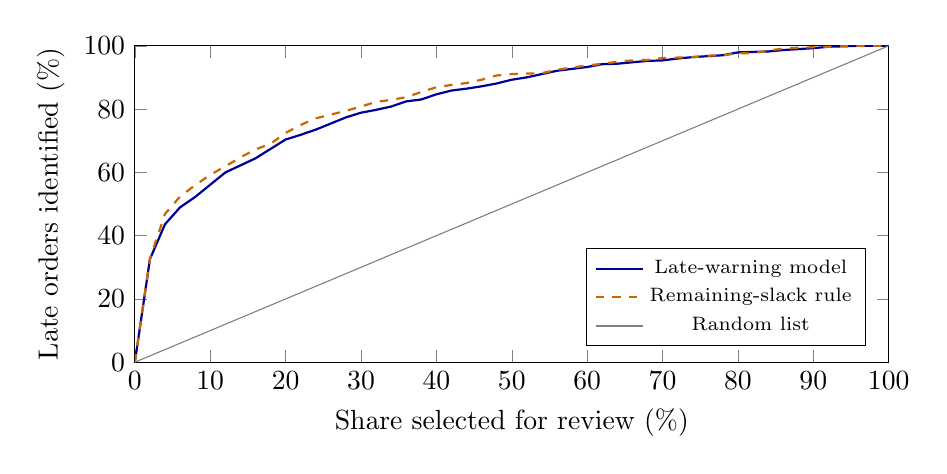
\begin{tikzpicture}
\begin{axis}[width=0.92\linewidth,height=5.6cm,xlabel={Share selected for review (\%)},ylabel={Late orders identified (\%)},
 xmin=0,xmax=100,ymin=0,ymax=100,legend style={at={(0.97,0.05)},anchor=south east,font=\scriptsize}]
\addplot[thick,blue!60!black,no marks] coordinates {(0.0,0.0000) (2.0,32.5893) (4.0,43.6012) (6.0,48.9583) (8.0,52.2321) (10.0,56.1012) (12.0,59.9702) (14.000000000000002,62.2024) (16.0,64.4345) (18.0,67.4107) (20.0,70.3869) (22.0,71.8750) (24.0,73.5119) (26.0,75.4464) (28.000000000000004,77.3810) (30.0,78.8690) (32.0,79.7619) (34.0,80.8036) (36.0,82.4405) (38.0,83.0357) (40.0,84.6726) (42.0,85.8631) (44.0,86.4583) (46.0,87.2024) (48.0,88.0952) (50.0,89.2857) (52.0,90.0298) (54.0,91.0714) (56.00000000000001,92.1131) (57.99999999999999,92.7083) (60.0,93.3036) (62.0,94.1964) (64.0,94.3452) (66.0,94.7917) (68.0,95.2381) (70.0,95.3869) (72.0,95.9821) (74.0,96.4286) (76.0,96.7262) (78.0,97.0238) (80.0,97.9167) (82.0,98.0655) (84.0,98.2143) (86.0,98.6607) (88.0,98.9583) (90.0,99.2560) (92.0,99.7024) (94.0,99.8512) (96.0,100.0000) (98.0,100.0000) (100.0,100.0000)};
\addlegendentry{Late-warning model}
\addplot[thick,orange!80!black,dashed,no marks] coordinates {(0.0,0.0000) (2.0,32.7381) (4.0,46.8750) (6.0,52.3810) (8.0,55.9524) (10.0,59.2262) (12.0,61.9048) (14.000000000000002,64.7321) (16.0,67.2619) (18.0,69.0476) (20.0,72.4702) (22.0,75.0000) (24.0,77.0833) (26.0,78.2738) (28.000000000000004,79.4643) (30.0,80.8036) (32.0,82.2917) (34.0,82.8869) (36.0,83.7798) (38.0,85.4167) (40.0,86.9048) (42.0,87.6488) (44.0,88.2440) (46.0,89.2857) (48.0,90.6250) (50.0,91.0714) (52.0,91.2202) (54.0,91.3690) (56.00000000000001,92.4107) (57.99999999999999,93.1548) (60.0,93.7500) (62.0,94.3452) (64.0,94.9405) (66.0,95.3869) (68.0,95.5357) (70.0,96.1310) (72.0,96.2798) (74.0,96.4286) (76.0,96.8750) (78.0,97.0238) (80.0,97.6190) (82.0,97.6190) (84.0,98.5119) (86.0,99.1071) (88.0,99.4048) (90.0,99.5536) (92.0,99.7024) (94.0,99.8512) (96.0,100.0000) (98.0,100.0000) (100.0,100.0000)};
\addlegendentry{Remaining-slack rule}
\addplot[thin,gray,no marks] coordinates {(0.0,0.0000) (2.0,2.0000) (4.0,4.0000) (6.0,6.0000) (8.0,8.0000) (10.0,10.0000) (12.0,12.0000) (14.000000000000002,14.0000) (16.0,16.0000) (18.0,18.0000) (20.0,20.0000) (22.0,22.0000) (24.0,24.0000) (26.0,26.0000) (28.000000000000004,28.0000) (30.0,30.0000) (32.0,32.0000) (34.0,34.0000) (36.0,36.0000) (38.0,38.0000) (40.0,40.0000) (42.0,42.0000) (44.0,44.0000) (46.0,46.0000) (48.0,48.0000) (50.0,50.0000) (52.0,52.0000) (54.0,54.0000) (56.00000000000001,56.0000) (57.99999999999999,58.0000) (60.0,60.0000) (62.0,62.0000) (64.0,64.0000) (66.0,66.0000) (68.0,68.0000) (70.0,70.0000) (72.0,72.0000) (74.0,74.0000) (76.0,76.0000) (78.0,78.0000) (80.0,80.0000) (82.0,82.0000) (84.0,84.0000) (86.0,86.0000) (88.0,88.0000) (90.0,90.0000) (92.0,92.0000) (94.0,94.0000) (96.0,96.0000) (98.0,98.0000) (100.0,100.0000)};
\addlegendentry{Random list}
\end{axis}
\end{tikzpicture}
% END GENERATED fig_gains
\caption{Test set (26 May--August 2018): share of late orders caught against share of orders reviewed, ranking within each purchase month.}
\label{fig:gains}
\end{figure}


\section*{Proposed Operations Workflow}
\textbf{Review workload.} In a day-by-day test-set replay, the \ActShare{}\% share flags a median of \FullDailyMedianFlagged{} parcels a day. Of the \FullDailyCaught{} late orders it identifies, \FullDailyBeforePromise{} are still open and before their promised date at 9am the next morning (Appendix Tables~\ref{tab:daily-replay} and~\ref{tab:daily-timing}). Operations would set its actual review capacity and adjust the list as late rates change.

\begin{enumerate}\setlength{\itemsep}{0pt}
\item \textbf{Each day at handover}, score every new parcel for late risk against its promised date and estimate its remaining delivery time. Rank the day's parcels for review the next morning. If the model is unavailable, rank by remaining slack instead.
\item \textbf{Each morning}, staff check the top of the list, up to a capacity operations chooses, with the remaining-time estimate to hand. Orders already past their date get an immediate update to the customer. For the rest, staff ask the carrier whether a faster service or another recovery option exists, and at what cost.
\item \textbf{Each month}, track whether the delivery estimate runs consistently long or short, the late rate, the length of Olist's promises, and how many flagged orders turn out late. A sustained change, or a change in how Olist sets promises, is the signal to review the model and list size. During a sharp shift, use the remaining-slack rule as a temporary ranking fallback until enough recent outcomes are available to retrain and check the model.
\end{enumerate}

\section*{Limitations}
\begin{itemize}\setlength{\itemsep}{0pt}
\item \textbf{Conditions change.} About \NormalLate{}\% of orders are late in ordinary months, but \BlackFridayLate{}\% were late around Black Friday and \FebMarLate{}\% in February--March 2018 (Appendix Figure~\ref{fig:monthly}). Olist's promises had stayed between \PromSpanMin{} and \PromSpanMax{} days a month from March 2017 to May 2018, then fell to \PromJul{} days in July and \PromAug{} in August 2018, shorter than in any earlier month. Models trained on one period carry its habits into the next: both regressions predicted deliveries about three days too long in the faster test set. That is why the workflow reviews performance monthly instead of fixing the models and the list size once.
\item \textbf{Cohort.} Results describe orders that were eventually delivered with a recorded carrier handover; cancelled and still-open orders have no outcome and are not covered.
\item \textbf{Available signals.} The supplied Olist tables lack carrier identity, live tracking events and capacity data. Route history and regional conditions are proxies, so the scores cannot identify the cause of an individual delay or react immediately to every disruption.
\item \textbf{Intervention outcomes.} Olist's data do not record carrier recovery options, their costs, or effects on delivery and reviews. The ranking results therefore show which orders could be prioritised, not the effect of contacting carriers or customers.
\end{itemize}

\section*{Conclusion}
At carrier handover, the regression gives staff a more accurate remaining-time estimate than the checkout forecast. The classifier prioritises late orders better than the remaining-slack rule in validation, but the rule ranks them better in the test set. A practical workflow would monitor both outputs and use the rule as a temporary fallback when the classifier's ranking weakens.

\section*{Declaration on the Use of AI}
Claude (Anthropic) and OpenAI Codex assisted with analysis code, figures and report drafting. The student authors are responsible for checking the calculations, citations and final submission.
\clearpage
\pagenumbering{arabic}
\renewcommand{\thepage}{R-\arabic{page}}
\begin{thebibliography}{99}\small\setlength{\itemsep}{0pt}
\bibitem{bergmeir2012} C.~Bergmeir and J.~M.~Ben\'itez. On the use of cross-validation for time series predictor evaluation. \emph{Information Sciences}, 2012. doi:10.1016/j.ins.2011.12.028.
\bibitem{breiman2001} L.~Breiman. Random forests. \emph{Machine Learning}, 45(1):5--32, 2001.
\bibitem{dearaujo2021} A.~C.~de Araujo and A.~Etemad. End-to-end prediction of parcel delivery time with deep learning for smart-city applications. \emph{IEEE Internet of Things Journal}, 8(23):17043--17056, 2021. doi:10.1109/JIOT.2021.3077007.
\bibitem{gibellini2024} F.~Gibellini, B.~van Gool, M.~Firat and S.~Bromuri. Estimating the time of arrival of a shipment with machine learning. \emph{ECAI 2024}, pp.~4681--4688. doi:10.3233/FAIA241064.
\bibitem{james2013} G.~James, D.~Witten, T.~Hastie and R.~Tibshirani. \emph{An Introduction to Statistical Learning}, Sec.~6.1.3, p.~214. Springer, 2013.
\bibitem{saito2015} T.~Saito and M.~Rehmsmeier. The precision-recall plot is more informative than the ROC plot when evaluating binary classifiers on imbalanced datasets. \emph{PLOS ONE}, 10(3):e0118432, 2015.
\bibitem{salari2022} N.~Salari, S.~Liu and Z.-J.~M.~Shen. Real-time delivery time forecasting and promising in online retailing: when will your package arrive? \emph{Manufacturing \& Service Operations Management}, 24(3):1421--1436, 2022.
\end{thebibliography}

\clearpage
\pagenumbering{arabic}
\renewcommand{\thepage}{A-\arabic{page}}
\appendix
\section{Prepared-table validation}
\label{app:gx}
Before the delivery-sequence exclusions, a Great Expectations (GX Core 1.24.0) suite checked the 96,470-row prepared order table. Its saved run passed all 35 expectations: eight identity, target and split checks; one exact-column-set check; 16 value-range checks; five category checks; and five missingness checks. Separate timestamp checks confirmed that fitting outcomes were recorded by the 26 May 2018 cutoff. The model comparison uses 96,272 orders after excluding 198 rows without a valid purchase--carrier--delivery sequence.

\begin{table}[ht]
\centering\small
\caption{Prepared-table validation and test-set feature checks. The 35 contract checks apply before the final sequence filter; monthly feature checks are separate diagnostics.}
\label{tab:gx}
\begin{tabular}{@{}lr@{}}
\toprule
Check & Saved result \\
\midrule
Identity, targets and split & 8/8 passed \\
Exact column set & 1/1 passed \\
Value ranges and categories & 21/21 passed \\
Documented missingness & 5/5 passed \\
Test-set monthly feature means outside training range & 5 of 21 \\
\bottomrule
\end{tabular}
\end{table}

The five out-of-range means are June freight, July promised days and freight, and August promised days and historical seller handover time. They document a change in the observed feature mix, not its cause. An exact column set can catch an unapproved predictor, but cannot establish when a historical value became known; the point-in-time feature construction is checked separately.

\section{Delivery context and diagnostics}
\label{app:diag}
\begin{table}[H]
\centering\small
\caption{Test-set ranking and top-\ActShare{}\% purchase-month review list. PR-AUC and ROC-AUC use all orders; precision, recall and F1 use the list.}
\label{tab:classifier-test}
\begin{tabular}{@{}lccccc@{}}
\toprule
& PR-AUC & ROC-AUC & Precision & Recall & F1 \\
\midrule
Late-warning model & \ClsTestPR{} & \ClsTestROC{} & \ClsTestPrec{}\% & \ClsTestRec{}\% & \ClsTestFone{} \\
Remaining-slack rule & \RuleTestPR{} & \RuleTestROC{} & \RuleTestPrec{}\% & \RuleTestRec{}\% & \RuleTestFone{} \\
Random list & \ClsTestLate{}\% & 0.50 & \ClsTestLate{}\% & \ActShare{}\% & --- \\
\bottomrule
\end{tabular}
\end{table}

\begin{table}[H]
\centering\small
\caption{Purchase-month test ranking at the illustrative \ActShare{}\% review share. Counts describe orders flagged for review, not carrier interventions.}
\label{tab:classifier-monthly}
\begin{tabular}{@{}lrrrr@{}}
\toprule
Month & Orders & Late orders & Flagged & Late caught \\
\midrule
May (from the 26th) & \TestMayOrders{} & \TestMayLateCount{} & \TestMayActed{} & \TestMayCaught{} \\
June & \TestJunOrders{} & \TestJunLateCount{} & \TestJunActed{} & \TestJunCaught{} \\
July & \TestJulOrders{} & \TestJulLateCount{} & \TestJulActed{} & \TestJulCaught{} \\
August & \TestAugOrders{} & \TestAugLateCount{} & \TestAugActed{} & \TestAugCaught{} \\
\bottomrule
\end{tabular}
\end{table}
% BEGIN GENERATED fig_classifier_windows -- refreshed by phase2_final_evidence.py
\begin{table}[H]
\centering\small
\caption{The selected classifier in each validation window. The late rate of each window is the PR-AUC of a random list.}
\label{tab:classifier-windows}
\begin{tabular}{@{}lrrrrr@{}}
\toprule
Window & Orders & Late rate & PR-AUC & ROC-AUC & Top-10\% precision \\
\midrule
W1 & 7,600 & 4.1\% & 0.378 & 0.815 & 21.6\% \\
W2 & 7,601 & 13.8\% & 0.430 & 0.778 & 44.8\% \\
W3 & 7,601 & 4.8\% & 0.282 & 0.756 & 16.6\% \\
W4 & 7,601 & 9.9\% & 0.370 & 0.785 & 36.0\% \\
W5 & 7,600 & 20.7\% & 0.502 & 0.768 & 61.7\% \\
\bottomrule
\end{tabular}
\end{table}
% END GENERATED fig_classifier_windows
% BEGIN GENERATED fig_split_summary -- refreshed by phase2_final_evidence.py
\begin{table}[H]
\centering\small
\caption{Descriptive scores for the chosen models. Training is scored in sample; validation averages five separately fitted chronological windows; the test set uses a model fitted on pre-test data. Late rates and case mixes differ, so the PR-AUC values are not a like-for-like learning curve.}
\label{tab:split-summary}
\begin{tabular}{@{}lrrr@{}}
\toprule
Metric & Training & Validation & Test set \\
\midrule
Checkout MAE (days) & 5.23 & 5.81 & 5.00 \\
Handover MAE (days) & 4.57 & 5.10 & 3.97 \\
Late warning PR-AUC & 0.374 & 0.392 & 0.489 \\
Late prevalence & 7.1\% & 10.7\% & 3.5\% \\
\bottomrule
\end{tabular}
\end{table}
% END GENERATED fig_split_summary
% BEGIN GENERATED fig_complete_daily_replay -- refreshed by phase2_final_evidence.py
\begin{table}[H]
\centering\small
\caption{Day-by-day replay of the chosen model, flagging the top \ActShare{}\% of handovers each day. Each row covers every valid handover in its calendar span. Counts show which orders would be flagged, not the effect of acting on them.}
\label{tab:daily-replay}
\begin{tabular}{@{}lrrrrrr@{}}
\toprule
Period & Active days & Orders & Late rate & Median flagged/day & Precision & Recall \\
\midrule
W1 & 45 & 7,262 & 3.6\% & 19 & 16.8\% & 47.9\% \\
W2 & 24 & 7,450 & 12.9\% & 36 & 39.5\% & 31.0\% \\
W3 & 33 & 7,685 & 5.7\% & 26 & 22.9\% & 41.0\% \\
W4 & 28 & 7,591 & 9.1\% & 32 & 29.6\% & 33.2\% \\
W5 & 29 & 7,357 & 21.9\% & 29 & 61.6\% & 28.7\% \\
Test set & 81 & 19,534 & 3.6\% & 27 & 19.5\% & 55.0\% \\
\bottomrule
\end{tabular}
\end{table}
% END GENERATED fig_complete_daily_replay
\begin{table}[H]
\centering\small
\caption{Test-set daily replay: next-morning timing for the late orders identified by the review list.}
\label{tab:daily-timing}
\begin{tabular}{@{}lr@{}}
\toprule
Status & Orders \\
\midrule
Late orders identified & \FullDailyCaught{} \\
Still open and before promised date at 9am & \FullDailyBeforePromise{} \\
Promised date already passed by 9am & \FullDailyExpiredCaught{} \\
\bottomrule
\end{tabular}
\end{table}

\textbf{Same-period diagnostic.} A secondary random five-fold validation and 20\% test yield checkout \(R^2\) \CheckoutRandValRSq{} / \CheckoutRandTestRSq{} (test MAE \CheckoutRandTestMAE{}) and handover \(R^2\) \HandoverRandValRSq{} / \HandoverRandTestRSq{} (test MAE \HandoverRandTestMAE{}). These interpolate within one period; their stronger scores illustrate the cost of temporal shift.
\begin{figure}[H]
\centering
% BEGIN GENERATED fig_monthly -- refreshed by phase2_final_evidence.py
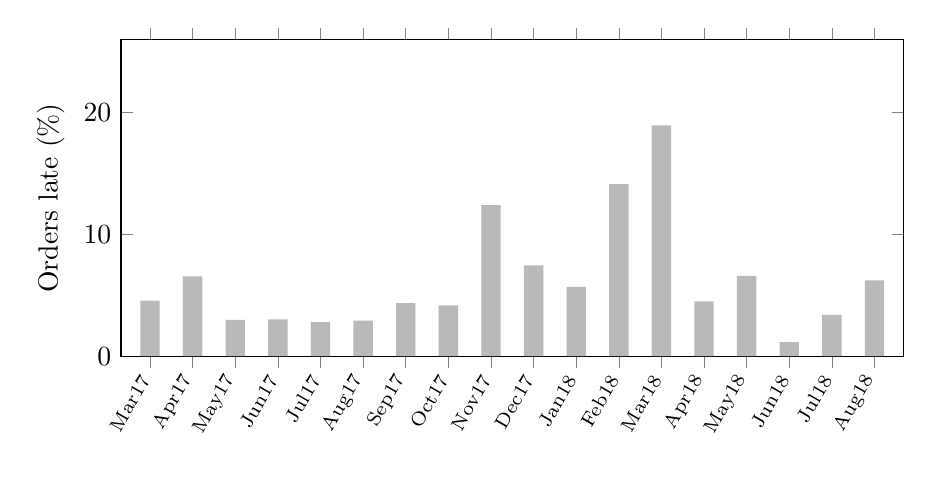
\begin{tikzpicture}
\begin{axis}[width=0.95\linewidth,height=5.6cm,ybar,bar width=7pt,ymin=0,ymax=26,ylabel={Orders late (\%)},
 symbolic x coords={Mar17,Apr17,May17,Jun17,Jul17,Aug17,Sep17,Oct17,Nov17,Dec17,Jan18,Feb18,Mar18,Apr18,May18,Jun18,Jul18,Aug18},xtick=data,x tick label style={rotate=60,anchor=east,font=\scriptsize},
 enlarge x limits=0.04]
\addplot[fill=gray!55,draw=none] coordinates {(Mar17,4.558) (Apr17,6.557) (May17,2.991) (Jun17,3.031) (Jul17,2.799) (Aug17,2.912) (Sep17,4.362) (Oct17,4.176) (Nov17,12.404) (Dec17,7.455) (Jan18,5.701) (Feb18,14.127) (Mar18,18.966) (Apr18,4.506) (May18,6.593) (Jun18,1.157) (Jul18,3.383) (Aug18,6.232)};
\end{axis}
\end{tikzpicture}
% END GENERATED fig_monthly
\caption{Share of orders late by purchase month. Black Friday (November 2017) and February--March 2018 stand out as the clearest swings in delivery conditions; the June--August 2018 test months at right were calmer at \ClsTestLate{}\% late.}
\label{fig:monthly}
\end{figure}


\begin{figure}[H]
\centering
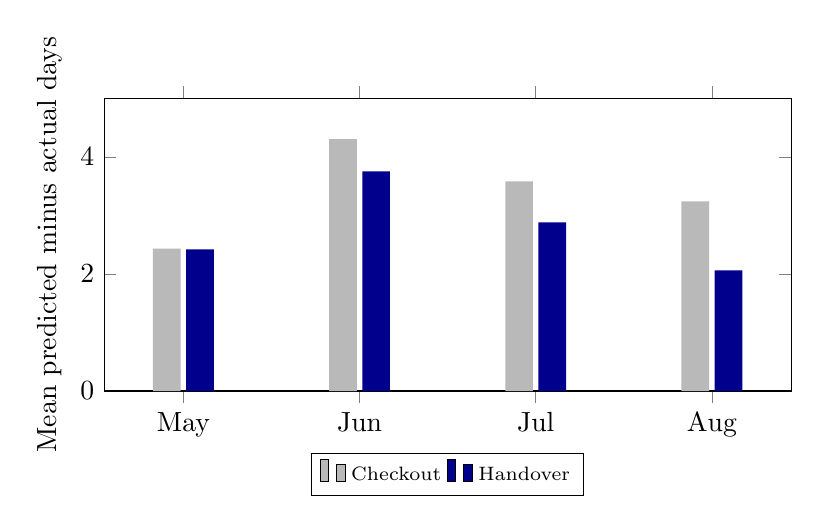
\begin{tikzpicture}
\begin{axis}[width=0.85\linewidth,height=5.3cm,ybar,bar width=10pt,ymin=0,ymax=5,
 symbolic x coords={May,Jun,Jul,Aug},xtick=data,enlarge x limits=0.15,
 ylabel={Mean predicted minus actual days},
 legend style={at={(0.5,-0.21)},anchor=north,legend columns=2,font=\scriptsize}]
\addplot[fill=gray!55,draw=none] coordinates {(May,2.43) (Jun,4.30) (Jul,3.58) (Aug,3.24)};
\addplot[fill=blue!55!black,draw=none] coordinates {(May,2.42) (Jun,3.75) (Jul,2.88) (Aug,2.06)};
\legend{Checkout,Handover}
\end{axis}
\end{tikzpicture}
\caption{Signed forecast error by purchase month in the test set (May starts on the 26th). Positive values mean predicted delivery is later than actual delivery. This diagnoses the shift to faster deliveries.}
\label{fig:test-bias}
\end{figure}

% BEGIN GENERATED fig_roc_pr -- refreshed by phase2_final_evidence.py
\begin{figure}[H]
\centering
\begin{minipage}{0.49\linewidth}\centering
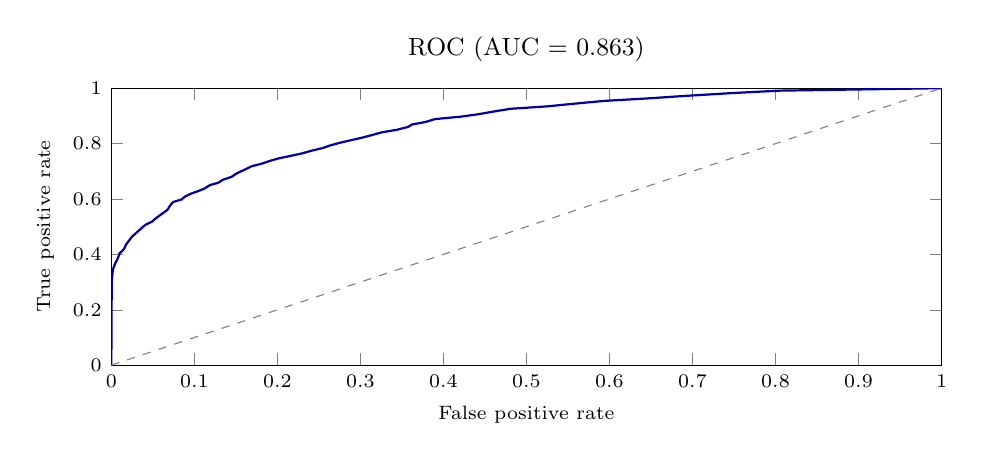
\begin{tikzpicture}
\begin{axis}[width=\linewidth,height=5.1cm,xmin=0,xmax=1,ymin=0,ymax=1,title style={font=\small},tick label style={font=\scriptsize},label style={font=\scriptsize},xlabel={False positive rate},ylabel={True positive rate},title={ROC (AUC = 0.863)}]
\addplot[thick,blue!65!black,no marks] coordinates {(0.0000,0.0000) (0.0005,0.2961) (0.0012,0.3244) (0.0019,0.3452) (0.0035,0.3586) (0.0047,0.3676) (0.0071,0.3810) (0.0089,0.3943) (0.0098,0.4033) (0.0135,0.4137) (0.0159,0.4226) (0.0175,0.4345) (0.0197,0.4435) (0.0227,0.4554) (0.0256,0.4658) (0.0300,0.4777) (0.0345,0.4896) (0.0378,0.4985) (0.0414,0.5074) (0.0488,0.5179) (0.0528,0.5283) (0.0580,0.5402) (0.0629,0.5506) (0.0676,0.5610) (0.0695,0.5699) (0.0718,0.5804) (0.0746,0.5893) (0.0846,0.5982) (0.0885,0.6086) (0.0957,0.6190) (0.1041,0.6280) (0.1117,0.6369) (0.1189,0.6503) (0.1293,0.6592) (0.1345,0.6696) (0.1450,0.6801) (0.1499,0.6905) (0.1559,0.6994) (0.1634,0.7098) (0.1696,0.7188) (0.1814,0.7277) (0.1915,0.7381) (0.2020,0.7470) (0.2166,0.7560) (0.2301,0.7649) (0.2425,0.7753) (0.2550,0.7842) (0.2634,0.7932) (0.2762,0.8036) (0.2890,0.8125) (0.3020,0.8214) (0.3152,0.8318) (0.3260,0.8408) (0.3437,0.8497) (0.3574,0.8601) (0.3623,0.8690) (0.3784,0.8780) (0.3899,0.8884) (0.4210,0.8973) (0.4426,0.9062) (0.4595,0.9152) (0.4807,0.9256) (0.5255,0.9345) (0.5558,0.9435) (0.5926,0.9539) (0.6444,0.9628) (0.6889,0.9717) (0.7462,0.9821) (0.8049,0.9911) (1.0000,1.0000)};
\addplot[thin,gray,dashed,no marks] coordinates {(0,0) (1,1)};
\end{axis}
\end{tikzpicture}
\end{minipage}\hfill
\begin{minipage}{0.49\linewidth}\centering
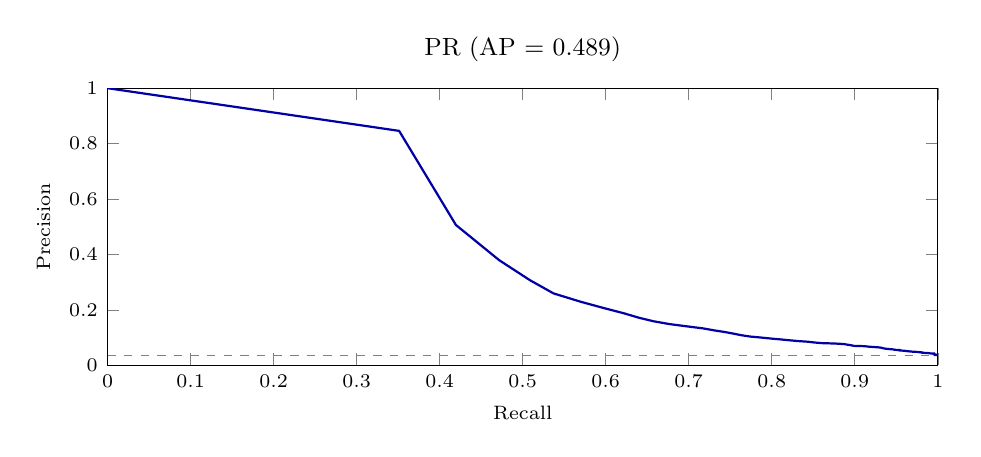
\begin{tikzpicture}
\begin{axis}[width=\linewidth,height=5.1cm,xmin=0,xmax=1,ymin=0,ymax=1,title style={font=\small},tick label style={font=\scriptsize},label style={font=\scriptsize},xlabel={Recall},ylabel={Precision},title={PR (AP = 0.489)}]
\addplot[thick,blue!65!black,no marks] coordinates {(0.0000,1.0000) (0.3512,0.8459) (0.4196,0.5063) (0.4717,0.3792) (0.5089,0.3067) (0.5372,0.2592) (0.5699,0.2291) (0.5982,0.2060) (0.6220,0.1874) (0.6399,0.1715) (0.6577,0.1586) (0.6771,0.1484) (0.6979,0.1403) (0.7173,0.1330) (0.7307,0.1258) (0.7440,0.1196) (0.7545,0.1137) (0.7634,0.1083) (0.7738,0.1036) (0.7872,0.0999) (0.7991,0.0963) (0.8110,0.0931) (0.8214,0.0900) (0.8318,0.0872) (0.8438,0.0848) (0.8512,0.0821) (0.8601,0.0798) (0.8765,0.0783) (0.8869,0.0764) (0.8914,0.0741) (0.8958,0.0720) (0.8988,0.0699) (0.9122,0.0687) (0.9167,0.0670) (0.9241,0.0655) (0.9301,0.0641) (0.9330,0.0625) (0.9345,0.0609) (0.9375,0.0595) (0.9420,0.0582) (0.9464,0.0571) (0.9479,0.0557) (0.9539,0.0548) (0.9539,0.0535) (0.9583,0.0525) (0.9613,0.0515) (0.9643,0.0505) (0.9673,0.0496) (0.9702,0.0487) (0.9762,0.0480) (0.9777,0.0471) (0.9807,0.0464) (0.9807,0.0455) (0.9836,0.0447) (0.9881,0.0441) (0.9896,0.0434) (0.9911,0.0427) (0.9955,0.0421) (0.9955,0.0414) (0.9955,0.0407) (0.9955,0.0400) (0.9955,0.0394) (0.9970,0.0388) (0.9970,0.0382) (0.9970,0.0376) (0.9970,0.0370) (1.0000,0.0365) (1.0000,0.0360) (1.0000,0.0355) (1.0000,0.0349)};
\addplot[thin,gray,dashed,no marks] coordinates {(0,0.0349) (1,0.0349)};
\end{axis}
\end{tikzpicture}
\end{minipage}
\caption{Final handover logistic classifier on 19,230 test-set orders (672 late). Curves are sampled points for display; AUC and average precision (AP) use all predictions. Dashed lines show random ranking. The top-\ActShare{}\% review list is drawn separately each month, so it is not a single point on these curves.}
\label{fig:roc-pr}
\end{figure}
% END GENERATED fig_roc_pr

% BEGIN GENERATED fig_confusion -- refreshed by phase2_final_evidence.py
\begin{table}[H]
\centering\small
\caption{Test-set confusion counts for the top-\ActShare{}\% monthly review list. Counts show who would be flagged, before any action is taken.}
\label{tab:app-confusion}
\begin{tabular}{@{}lrr@{}}
\toprule
& Actually late & Actually on time \\
\midrule
Selected for review & 377 & 1,547 \\
Not selected & 295 & 17,011 \\
\bottomrule
\end{tabular}
\end{table}
% END GENERATED fig_confusion

At this review share, MCC is \ClsTestMCC{} (zero indicates no association between selection and lateness).

\section{Monthly retraining check}
\label{app:monthly-retraining}
This check asks whether refitting the backlog-augmented logistic classifier each month helps it respond to shorter promises. Each method reviews the top 10\% of handovers within each handover month.

\begin{table}[H]
\centering\small
\caption{Late orders identified at the same review share. Validation compares monthly with quarterly refitting; the test set compares monthly refitting with the model fitted once in May.}
\label{tab:monthly-retraining}
\begin{tabular}{@{}lrrr@{}}
\toprule
Period & Monthly model & Comparison model & Remaining-slack rule \\
\midrule
Validation replay & \MonthlyValCaught{} & \QuarterlyValCaught{} & \MonthlyRuleValCaught{} \\
Test set & \MonthlyTestCaught{} & \FrozenTestCaught{} & \MonthlyRuleTestCaught{} \\
\bottomrule
\end{tabular}
\end{table}
Monthly refitting finds more late orders than the comparison model, but the rule still finds more in the test set. The main report ranks the test list by purchase month; this check ranks by handover month, so the counts differ slightly. Delivery outcomes become available only after arrival, which limits how quickly a refresh can respond to a sharp change.

\section{Full configuration tables}
% BEGIN GENERATED fig_appendix_regression -- refreshed by phase2_final_evidence.py
\begin{table}[H]
\centering\small
\caption{Every regression candidate, mean over five validation windows.}
\label{tab:app-regression}
\begin{tabular}{@{}lllrrr@{}}
\toprule
Stage & Candidate & Family & MAE & RMSE & $R^2$ \\
\midrule
Checkout & mean\_baseline & mean & 7.215 & 10.671 & -0.078 \\
Checkout & linear\_baseline & linear & 5.860 & 9.464 & 0.155 \\
Checkout & ridge\_1 & ridge & 5.858 & 9.462 & 0.156 \\
Checkout & ridge\_10 & ridge & 5.848 & 9.451 & 0.158 \\
Checkout & ridge\_100 & ridge & 5.809 & 9.398 & 0.167 \\
Checkout & tree\_baseline & tree & 7.787 & 12.344 & -0.472 \\
Checkout & tree\_depth6 & tree & 5.933 & 9.505 & 0.144 \\
Checkout & forest\_leaf20 & forest & 5.783 & 9.340 & 0.176 \\
Checkout & boost\_baseline & boost & 5.830 & 9.452 & 0.155 \\
Checkout & boost\_slow & boost & 5.816 & 9.444 & 0.157 \\
Handover & mean\_baseline & mean & 7.215 & 10.671 & -0.078 \\
Handover & elapsed\_plus\_route\_baseline & rule & 5.304 & 8.396 & 0.337 \\
Handover & linear\_baseline & linear & 5.146 & 8.472 & 0.327 \\
Handover & ridge\_1 & ridge & 5.145 & 8.470 & 0.327 \\
Handover & ridge\_10 & ridge & 5.136 & 8.460 & 0.329 \\
Handover & ridge\_100 & ridge & 5.099 & 8.406 & 0.338 \\
Handover & tree\_baseline & tree & 6.840 & 11.625 & -0.330 \\
Handover & tree\_depth6 & tree & 5.313 & 8.633 & 0.299 \\
Handover & forest\_leaf20 & forest & 5.346 & 8.808 & 0.270 \\
Handover & boost\_baseline & boost & 5.214 & 8.651 & 0.297 \\
Handover & boost\_slow & boost & 5.215 & 8.666 & 0.294 \\
Handover & voting\_family\_winners & voting & 5.107 & 8.471 & 0.327 \\
\bottomrule
\end{tabular}
\end{table}
% END GENERATED fig_appendix_regression
% BEGIN GENERATED fig_appendix_classifier -- refreshed by phase2_final_evidence.py
\begin{table}[H]
\centering\small
\caption{Every classifier candidate, mean over five validation windows (handover stage).}
\label{tab:app-classifier}
\begin{tabular}{@{}lrrr@{}}
\toprule
Candidate & PR-AUC & ROC-AUC & Recall at top 10\% \\
\midrule
logistic\_unregularized & 0.371 & 0.747 & 0.357 \\
logistic\_c1 & 0.377 & 0.754 & 0.355 \\
logistic\_c1\_bal & 0.369 & 0.747 & 0.354 \\
logistic\_c0.01 & 0.392 & 0.780 & 0.373 \\
logistic\_c0.01\_bal & 0.385 & 0.772 & 0.362 \\
logistic\_c0.1 & 0.386 & 0.769 & 0.367 \\
logistic\_c0.1\_bal & 0.375 & 0.755 & 0.356 \\
logistic\_c10 & 0.373 & 0.749 & 0.354 \\
logistic\_c10\_bal & 0.367 & 0.744 & 0.352 \\
tree\_plain & 0.140 & 0.567 & 0.222 \\
tree\_d4\_l20 & 0.272 & 0.654 & 0.273 \\
tree\_d4\_l100 & 0.269 & 0.654 & 0.272 \\
tree\_d6\_l20 & 0.296 & 0.690 & 0.288 \\
tree\_d6\_l100 & 0.305 & 0.701 & 0.301 \\
tree\_d8\_l20 & 0.301 & 0.691 & 0.278 \\
tree\_d8\_l100 & 0.320 & 0.705 & 0.314 \\
tree\_d12\_l20 & 0.299 & 0.654 & 0.287 \\
tree\_d12\_l100 & 0.314 & 0.669 & 0.313 \\
forest\_l5\_sqrt & 0.369 & 0.737 & 0.346 \\
forest\_l5\_half & 0.354 & 0.723 & 0.332 \\
forest\_l20\_sqrt & 0.373 & 0.744 & 0.352 \\
forest\_l20\_half & 0.364 & 0.730 & 0.345 \\
forest\_l50\_sqrt & 0.372 & 0.747 & 0.347 \\
forest\_l50\_half & 0.369 & 0.737 & 0.349 \\
boost\_lr0.03\_n200\_l20 & 0.363 & 0.741 & 0.343 \\
boost\_lr0.03\_n200\_l100 & 0.353 & 0.734 & 0.336 \\
boost\_lr0.03\_n500\_l20 & 0.358 & 0.736 & 0.334 \\
boost\_lr0.03\_n500\_l100 & 0.343 & 0.725 & 0.326 \\
boost\_lr0.1\_n200\_l20 & 0.345 & 0.732 & 0.327 \\
boost\_lr0.1\_n200\_l100 & 0.338 & 0.725 & 0.319 \\
boost\_lr0.1\_n500\_l20 & 0.336 & 0.717 & 0.315 \\
boost\_lr0.1\_n500\_l100 & 0.329 & 0.715 & 0.314 \\
\bottomrule
\end{tabular}
\end{table}
% END GENERATED fig_appendix_classifier

\end{document}
